\chapter{Базовые сведения}
 В данной главе описаны основные аспекты процесса разработки приложений с использованием gtkmm. Для их демонстрации приведен простой работоспособный пример кода. Однако, это всего лишь вводное описание, поэтому вам придется рассмотреть остальные главы для получения более подробной информации.

Ваши знания из области языка программирования C++ помогут вам в работе с gtkmm, также, как и при работе с любой другой библиотекой. Если мы не предупреждаем об обратном, вы можете быть уверенными в том, что классы gtkmm ведут себя аналогично любому другому классу языка C++, причем вы можете использовать известные вам техники работы с классами языка C++ для работы с классами gtkmm. 

\section{Простой пример}
В начале нашего вводного описания gtkmm рассмотрим простейшую из возможных программ. Эта программа создает пустое окно размером 200 x 200 пикселей. 

Файл base.cpp (Предназначен для использования совместно с gtkmm 3, а не с gtkmm 2): 
\begin{lstlisting}[language=C++]
#include <gtkmm.h>

int main(int argc, char *argv[])
{
	Glib::RefPtr<Gtk::Application> app = Gtk::Application::create(argc, argv,
		"org.gtkmm.examples.base");
	Gtk::Window window;
	window.set_default_size(200, 200);

	return app->run(window);
}

\end{lstlisting}
Теперь рассмотрим каждую из строк примера. 
\begin{lstlisting}[language=C++]
#include <gtkmm.h>
\end{lstlisting}
Каждая из использующих gtkmm программ должна подключать определенные заголовочные файлы gtkmm; подключение заголовочного файла gtkmm.h позволяет подключить все заголовочные файлы из состава gtkmm. Обычно использование этого заголовочного файла не является удачной идеей, так как происходит подключение около мегабайта заголовочных файлов, но в случае простых программ это допустимо. 

Следующее объявление: 
\begin{lstlisting}[language=C++]
Glib::RefPtr<Gtk::Application> app = Gtk::Application::create(argc, argv, "org.gtkmm.examples.base");
\end{lstlisting}
позволяет создать объект \textbf{Gtk::Application}, сохраняемый с помощью умного указателя \textbf{RefPtr}. Это действие должно выполняться во всех приложениях на основе gtkmm. Метод \textbf{create()} этого объекта производит инициализацию gtkmm и проверку аргументов, передаваемых вашей программе в командной строке с одновременным поиском таких стандартных параметров, как --display. Он извлекает стандартные параметры из списка параметров, после чего в списке остаются только неизвестные параметры, которые могут быть использованы или проигнорированы на уровне приложения. Такой алгоритм работы позволяет быть уверенным в том, что все приложения на основе gtkmm будут принимать один и тот же набор стандартных аргументов. 

С помощью следующих двух строк кода создается окно и устанавливается его стандартный (начальный) размер: 
\begin{lstlisting}[language=C++]
Gtk::Window window;
window.set_default_size(200, 200);
\end{lstlisting}
С помощью последней строки кода осуществляется показ окна и вход в главный цикл обработки событий, который прекратит свою работу в момент, когда окно будет закрыто. После этого ваша функция main() сможет вернуть соответствующий код удачного завершения работы приложения или ошибки. 
\begin{lstlisting}[language=C++]
return app->run(window);
\end{lstlisting}
После сохранения исходного кода в файле с именем simple.cc вы сможете скомпилировать описанную выше программу с помощью компилятора gcc, воспользовавшись следующей командой:
\begin{lstlisting}[language=bash]
g++ simple.cc -o simple `pkg-config gtkmm-3.0 --cflags --libs`
\end{lstlisting}
Следует отметить, что вы должны экранировать вызов pkg-config с помощью обратных кавычек. Обратные кавычки позволяют командной оболочке выполнить команду внутри них и использовать вывод этой команды в качестве части основной команды. Также следует отметить, что имя файла simple.cc должно быть расположено перед вызовом pkg-config в рамках основной команды. 

Для cmake приблизительно будет выглядеть так: 
\begin{lstlisting}[language=bash]
cmake_minimum_required(VERSION 3.10)
project(windowExample)
set(CMAKE_CXX_STANDARD 14)

find_package(PkgConfig)
pkg_check_modules(GTKMM gtkmm-3.0)

link_directories(
${GTKMM_LIBRARY_DIRS}  )

include_directories(
${GTKMM_INCLUDE_DIRS}  )

add_executable(windowExample main.cpp MainWindow.cpp AddIPModal.cpp AddIPModal.h)

target_link_libraries(windowExample ${GTKMM_LIBRARIES})
\end{lstlisting}

\section{Заголовочные файлы и связывание}
 Хотя мы и показали команду компиляции простого примера, при разработке реальных приложений вам следует использовать инструменты automake и autoconf таким образом, как это описано в работе G. V. Vaughan и других авторов под названием "Autoconf, Automake, Libtool". Исходный код примеров, использованных в данной книге, включен вместе с соответствующими файлами сборки в пакет gtkmm, поэтому впредь мы не будем приводить команды сборки. Для осуществления сборки примера вам всего лишь потребуется найти соответствующую директорию и выполнить в ней команду make.

Для упрощения компиляции мы используем инструмент pkg-config, вспомогательные файлы для которого присутствуют во всех (корректных) установках gtkmm. Эта программа "знает" о том, какие параметры компилятора необходимы для компиляции программ, использующих gtkmm. Параметр --cflags сообщает pkg-config о необходимости вывода списка директорий с подключаемыми заголовочными файлами для того, чтобы компилятор имел возможность найти необходимые файлы; с помощью параметра --libs осуществляется запрос списка библиотек которые будут связываться приложением, а также директорий, в которых компилятор сможет найти их. Испытайте соответствующие команды в командой оболочке для того, чтобы узнать результаты их выполнения в вашей системе.
Однако, гораздо проще использовать макрос PKG\_CHECK\_MODULES() в стандартном файле configure.ac в случае работы с autoconf и automake. Пример использования:

PKG\_CHECK\_MODULES([MYAPP], [gtkmm-3.0 >= 3.0.0])

Это объявление позволяет проверить наличие gtkmm в системе и установить значения макросов MYAPP\_LIBS и MYAPP\_CFLAGS, которые будут использоваться в ваших файлах Makefile.am.

Текущий стабильный API носит имя gtkmm-3.0. Ранее использовалась устаревшая на данный момент версия API с именем gtkmm-2.4, которая сейчас может быть установлена параллельно с другими версиями. Существовало несколько версий gtkmm-2.4, таких как gtkmm-2.10 и при этом также будет выпущено несколько версий API gtkmm-3.0. Следует учесть, что имя API не меняется при выпуске каждой версии, так как в противном случае каждая из версий должна быть несовместимой с другими на уровне API и ABI. Теоретически в будущем будет выпущена версия API gtkmm-4.0, которая сможет устанавливаться параллельно с gtkmm-3.0 без оказания влияния на существующие приложения.

Следует отметить, что в том случае, если вы используете дополнительные модули в дополнение к gtkmm-3.0, они должны быть отделены пробелами, а не запятыми.

На ресурсе opensimus можно найти документ с базовой информацией об инструментах automake и autoconf. 

\section{Виджеты}
 Приложения на основе gtkmm состоят из окон, содержащих такие виджеты, как кнопки и поля ввода текста. В некоторых других системах виджеты называются "элементами управления". Каждому из виджетов в окнах вашего приложения соответствует объект языка программирования C++ в коде вашего приложения. Таким образом, вам нужно всего лишь использовать метод класса вашего виджета для воздействия на состояние видимого виджета.
Виджеты размещаются внутри таких контейнерных виджетов, как фреймы и наборы страниц с вкладками, формируя иерархию из виджетов, расположенных в других виджетах. Некоторые из этих контейнерных виджетов, такие, как представленные классом Gtk::Grid не являются видимыми - они существуют только для того, чтобы была возможность размещения других виджетов. Ниже приведен пример кода, предназначенного для добавления 2 виджетов-кнопок, представленных классом Gtk::Button, в контейнерный виджет, представленный классом Gtk::Box:
\begin{lstlisting}[language=C++]
m_box.pack_start(m_Button1);
m_box.pack_start(m_Button2);
\end{lstlisting}
а здесь представлен способ добавления виджета, представленного классом Gtk::Box и содержащего эти кнопки, в контейнерный виджет, представленный классом Gtk::Frame и имеющий видимую рамку и заголовок:
\begin{lstlisting}[language=C++]
m_frame.add(m_box);
\end{lstlisting}


В большей части глав данной книги рассматриваются определённые виджеты. Обратитесь к главе "Контейнерные виджеты" для получения более подробной информации о методах упаковки виджетов в контейнерные виджеты.

Хотя вы и можете задать параметры размещения и отображения виджетов на уровне кода на языке программирования C++, проектирование интерфейсов с использованием инструмента Glade и загрузка их в процессе работы приложения с помощью класса Gtk::Builder, скорее всего, покажется вам более удобным методом разработки пользовательских интерфейсов. Поэтому вам также следует обратить внимание на главу "Glade и Gtk::Builder".

Хотя экземпляры классов виджетов gtkmm и характеризуются такими же временами жизни и областями действия, как экземпляры других классов языка программирования C++, gtkmm предоставляет дополнительную возможность для экономии времени, применение которой вы можете увидеть в некоторых примерах. Метод Gtk::manage() позволяет сообщить механизму управления памятью о том, что виджетом владеет контейнер, в котором он размещён. Эта возможность позволяет вам создать виджет с помощью оператора new, поместить его в контейнер и забыть о его удалении. Подробнее о техниках управления памятью в gtkmm вы можете узнать, обратившись к главе "Управление памятью". 

\section{Сигналы}
 gtkmm, как и большинство тулкитов для построения графического пользовательского интерфейса управляется событиями. В момент наступления события, такого, как нажатие кнопки мыши, виджет, в области которого было осуществлено нажатие, осуществит генерацию соответствующего сигнала. Каждый виджет имеет отдельный набор сигналов, которые он может генерировать. Для того, чтобы в результате нажатия на кнопку выполнялось действие мы устанавливаем обработчик сигнала, который будет захватывать сигнал "clicked" ("нажата") от кнопки.
gtkmm использует библиотеку libsigc++ для реализации механизма сигналов. Ниже приведен пример строки кода, предназначенной для соединения сигнала "clicked" представленного классом Gtk::Button виджета с обработчиком сигнала с названием "on\_button\_clicked":
\begin{lstlisting}[language=C++]
m_button1.signal_clicked().connect( sigc::mem_fun(*this,
&HelloWorld::on_button_clicked) );
\end{lstlisting}

Для получения более подробной информации о сигналах, следует обратиться к приложению.

Если же вас интересует информация о способе реализации ваших собственных сигналов вместо простого соединения с уже существующими в рамках gtkmm сигналами, вам следует обратиться к следующему приложению. 
\section{Glib::ustring}
 Вы можете удивиться, когда узнаете, что gtkmm не использует класс std::string в своих интерфейсах. Вместо него используется класс Glib::ustring, который является настолько похожим и устроен аналогично упомянутому классу, что вы на самом деле можете считать, что каждый класс Glib::ustring на самом деле является классом std::string и проигнорировать оставшуюся часть данного раздела. Но вам все же следует прочитать раздел до конца в том случае, если вы планируете использовать в своем приложении языки, отличные от английского.

Класс std::string использует 8 бит для кодирования каждого символа, но 8 бит не достаточно для кодирования символов таких языков, как арабский, китайский и японский. Хотя методы кодирования символов таких языков и были описаны Консорциумом Unicode, языки программирования C и C++ до сегодняшнего дня не предоставляют каких-либо стандартизированных механизмов для работы с кодировкой Unicode. Разработчики GTK+ и GNOME решили реализовать поддержку кодировки Unicode, реализовав механизмы для работы с кодировкой UTF-8, которые и используются классом Glib::ustring. Он предоставляет практически тот же интерфейс, что и класс std::string с дополнительными функциями для конвертирования данных из представления и в представление класса std::string.

Одно из достоинств кодировки UTF-8 заключается в том, что вы можете не использовать ее тогда, когда не хотите, поэтому вам не придется модифицировать весь ваш код одномоментно. Класс std::string будет работать и с 7-битными строками в кодировке ASCII. Но после начала локализации вашего приложения для поддержки таких языков, как, например, китайский, вы столкнетесь со странными ошибками и, возможно, с аварийными завершениями работы приложения. В этом случае все, что вам потребуется - это начать использовать класс Glib::ustring вместо стандартного.

Следует учесть, что кодировка UTF-8 не является совместимой с такими 8-битными кодировками, как ISO-8859-1. К примеру, немецкие умляуты не находятся в диапазоне символов ASCII и требуют более одного байта для кодирования с использованием кодировки UTF-8. Если ваш код содержит строку с 8-битными символами, вам придется преобразовать их в кодировку UTF-8 (т.е., баварское приветствие "Grüß Gott" будет преобразовано к виду "Gr\\xC3\\xBC\\xC3\\x9F Gott").

Вам следует избегать использования арифметических действий с указателями в стиле языка программирования C, а также использования таких функций, как strlen(). В кодировке UTF-8 для кодирования символа может потребоваться от 1 до 6 байт, поэтому невозможно точно сказать, будет ли следующий байт представлять следующий символ. Класс Glib::ustring заботится об обработке данных символьных последовательностей, поэтому вы можете использовать такие методы, как Glib:ustring::substr(), производя расчеты в символах вместо байт.

В отличие от используемого в Windows решения, заключающегося в применении кодировки Unicode UCS-2, описанная кодировка не требует каких-либо специальных параметров компиляции для обработки символов строк и ее применение не приводит к появлению исполняемых файлов и библиотек с поддержкой кодировки Unicode, которые не совместимы с программными компонентами, поддерживающими кодировку ASCII.

Справочная информация

Обратитесь к разделу "Интернационализация" для получения более подробной информации о работе с символами строк, использующих кодировку UTF-8. 

\section{Промежуточные типы}
 Некоторые связанные с gtkmm API используют промежуточные контейнеры для данных, такие, как Glib::StringArrayHandle вместо таких специальных контейнеров из стандартной библиотеки языка программирования C++, как std::vector или std::list, хотя на уровне gtkmm начиная с gtkmm 3.0 используется исключительно класс std::vector.
Вы не должны декларировать эти типы самостоятельно. Вместо них вы должны использовать тот контейнер из стандартной библиотеки языка программирования C++, который предпочитаете. После этого на уровне gtkmm будет осуществлено преобразование типов. Ниже приведены примеры упомянутых промежуточных типов:
\begin{itemize}
	\item Вместо Glib::StringArrayHandle или Glib::ArrayHandle<Glib::ustring> следует  использовать std::vector<Glib::ustring>, std::list<Glib::ustring>, const char*[] и.т.д.
	\item Вместо Glib::ListHandle<Gtk::Widget*> следует использовать std::vector<Gtk::Widget*>, std::list<Gtk::Widget*> и.т.д.
	\item Вместо Glib::SListHandle<Gtk::Widget*> следует использовать std::vector<Gtk::Widget*>, std::list<Gtk::Widget*> и.т.д.
	
\end{itemize}

\section{Смешивание API языков C и С++}
 Вы можете использовать API языка C, которые на данный момент не имеют соответствующих интерфейсов на уровне языка C++. Обычно использование API языка C из приложения, разработанного с использованием языка C++, не является большой проблемой и gtkmm способствует этому, предоставляя доступ к расположенному уровнем ниже объекту языка C, а также предоставляя простой способ создания обертки для объекта на языке C++, предназначенной для работы с рассматриваемым объектом языка C, благодаря тому, что API языка C также основывается на системе GObject.
Для использования объекта gtkmm совместно с функцией языка C, которая принимает экземпляр класса GObject языка C, используйте функцию gobj(), позволяющую получить указатель на расположенный уровнем ниже экземпляр класса GObject. Например:

\begin{lstlisting}[language=C++]
Gtk::Button* button = new Gtk::Button("Example");
gtk_button_do_something_new(button->gobj());
\end{lstlisting}

Для получения экземпляра класса gtkmm из экземпляра класса GObject языка C используйте функцию Glib::wrap(). Например:

\begin{lstlisting}[language=C++]
GtkButton* cbutton = get_a_button();
Gtk::Button* button = Glib::wrap(cbutton);
\end{lstlisting}

\section{Приложение Hello World на основе gtkmm}
 Сейчас мы обладаем достаточными знаниями для рассмотрения реального примера. В соответствии со старой традицией из области компьютерных наук, мы будем исследовать приложение Hello World, созданное на основе gtkmm:

Исходный код

Файл helloworld.h (Для использования совместно с gtkmm 3, а не с gtkmm 2) 
\begin{lstlisting}[language=C++]
#ifndef GTKMM_EXAMPLE_HELLOWORLD_H
#define GTKMM_EXAMPLE_HELLOWORLD_H

#include <gtkmm/button.h>
#include <gtkmm/window.h>

class HelloWorld : public Gtk::Window
{
public:
	HelloWorld();
	virtual ~HelloWorld();

protected:
	
	void on_button_clicked();


	Gtk::Button m_button;
};

#endif 
\end{lstlisting}
Файл helloworld.cpp (Для использования совместно с gtkmm 3, а не с gtkmm 2) 
\begin{lstlisting}[language=C++]
#include "helloworld.h"
#include <iostream>

HelloWorld::HelloWorld()
	: m_button("Hello World")   
{
	
	set_border_width(10);
	
	
	m_button.signal_clicked().connect(sigc::mem_fun(*this,
	&HelloWorld::on_button_clicked));
	
	
	add(m_button);
	

	m_button.show();
}

HelloWorld::~HelloWorld()
{
}

void HelloWorld::on_button_clicked()
{
	std::cout << "Hello World" << std::endl;
}

\end{lstlisting}
Файл main.cc (Для использования совместно с gtkmm3, а не с gtkmm 2) 
\begin{lstlisting}[language=C++]
#include "helloworld.h"
#include <gtkmm/application.h>

int main (int argc, char *argv[])
{
	Glib::RefPtr<Gtk::Application> app = Gtk::Application::create(argc, argv, "org.gtkmm.example");
	
	HelloWorld helloworld;
	
	
	return app->run(helloworld);
}
\end{lstlisting}
Попробуйте скомпилировать и запустить приложение перед тем, как двигаться дальше. Вы должны увидеть что-то похожее на это:


\begin{figure}[h]
	\center{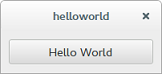
\includegraphics[width=1\linewidth]{31}}
	\caption{Hello world.}
	\label{ris:image}
\end{figure}
Довольно устрашающе, да? Давайте разбираться с кодом. Для начала класс HelloWorld: 
\begin{lstlisting}[language=C++]
class HelloWorld : public Gtk::Window
{

public:
	HelloWorld();
	virtual ~HelloWorld();
	
protected:
	virtual void on_button_clicked();
	Gtk::Button m_button;
};
\end{lstlisting}
Этот класс содержит реализацию функций окна "Hello World". Он наследуется от класса Gtk::Window и имеет единственный дочерний класс Gtk::Button. Мы решили использовать конструктор для выполнения всей работы по инициализации окна, включая установку обработчиков сигналов. Ниже приведен этот код с исключенными комментариями: 

\begin{lstlisting}[language=C++]
HelloWorld::HelloWorld()
:
m_button ("Hello World")
{
	set_border_width(10);
	m_button.signal_clicked().connect(sigc::mem_fun(*this,
	&HelloWorld::on_button_clicked));
	add(m_button);.
	m_button.show();
}
\end{lstlisting}
 Заметьте, что мы использовали объявление инициализации для вывода надписи "Hello World" на кнопке, представленной объектом m\_button.

После мы вызвали метод set\_border\_width() класса Gtk::Window. Этот метод позволяет установить ширину пространства между сторонами окна и виджетом, находящимся в окне.

После этого мы установили обработчик для сигнала "clicked" объекта m\_button. Он выводит дружественное приветствие в поток стандартного вывода (stdout).

Впоследствии мы использовали метод add() класса Gtk::Window для упаковки виджета, представленного объектом m\_button, в виджет, представленный объектом окна helloworld. (Метод add() помещает виджет, представленный экземпляром класса Gtk::Widget, в виджет, представленный экземпляром класса Gtk::Window, но не позволяет показать виджет. Виджеты в gtkmm обычно невидимы сразу же после создания - для их показа необходимо вызывать метод show(), что мы и делаем в следующей строке.

А теперь давайте рассмотрим функцию main() нашей программы. Эта функция с исключенными комментариями приведена ниже: 
\begin{lstlisting}[language=C++]
int main(int argc, char** argv)
{
	Glib::RefPtr<Gtk::Application> app = Gtk::Application::create(argc, argv, 		"org.gtkmm.example");
	
	HelloWorld helloworld;
	return app->run(helloworld);
}
\end{lstlisting}
 Для начала мы создаем объект с именем app, хранимый в умном указателе RefPtr. Это экземпляр класса Gtk::Application. Каждая программа на основе gtkmm должна иметь один такой объект. Мы передаем наши аргументы командной строки в качестве параметров его метода create(). Он обрабатывает те аргументы, которые пожелает, и оставляет вам все остальные, как мы и говорили ранее.

После этого мы создаем объект на основе нашего класса HelloWorld, конструктор которого не принимает никаких аргументов, но пока это не заметно. Когда мы вызываем метод Gtk::Application::run(), передавая экземпляр класса Gtk::Window приложения HelloWorld, происходит показ окна и запуск цикла обработки событий gtkmm. В процессе работы цикл обработки событий gtkmm ожидает действий от пользователя и отвечает на них соответствующим образом. В момент, когда пользователь закрывает окно, метод run() возвращает управление, что приводит к исполнению последней строки кода нашей функции main(). После этого работа приложения завершается. 